\chapter{氮氧化物排放量软测量}
\label{chap:softsensor}
\section{概述}

如~\ref{sec:nox_measure_now}~节所述,现场的~\ce{NOx}~测量装置存在一系列的问题,这些问题导致脱硝回路的异常运行。现场先进控制系统的投运取得了良好的控制效果,但其控制效果依赖于各测量点的测量品质,且先进控制系统在测点品质差的时候会自动切换回手动控制。因此,为了保障现场~\ce{NOx}~实时监测和脱硝系统的正常运行,必须利用更好的测量方法来测量~\ce{NOx}~排放量。利用软测量技术建立~\ce{NOx}~模型,既可以与传感器并行运行,作为其测量值的补充,减少测量滞后和噪声的影响;也可以在传感器故障、更换、维护、重新标定期间作为维持系统正常运行的测量装置。另外,由于现场测点限制,目前脱硝回路控制的策略只是将~\ce{NOx}~排放量作为回路的反馈值,构成闭环控制。由软测量模型可以获得脱硝前的~\ce{NOx}~含量,作为控制器的参考输入量,提高回路控制水平。

软测量的设计一般分为如下几步\cite{Fortuna2007Soft}:
\begin{enumerate}
\item {数据收集与预处理;}
\item {模型和输入变量选择;}
\item {模型辨识;}
\item {模型校验。}
\end{enumerate}

现场数据库存储了大量的循环流化床锅炉运行数据,这为软测量的设计提供了基础。由于回归模型算法简单、计算速度快,最有可能作为在线软测量模型。通过分析~\ce{NOx}~生成和脱硝机理选择输入变量并建立回归模型,考虑模型要跟上工况变化,结合滚动窗思想建立在线更新的软测量模型。最后,讨论窗口大小和滑动距离对软测量模型性能的影响。


\section{输入变量}
\subsection{建立输入变量集}

由于燃烧生成的氮氧化物主要是~\ce{NO},且很多其他氮氧化物可由~\ce{NO}~进一步反应得到,大部分研究都针对~\ce{NO}~的生成来描述~\ce{NOx}~生成机理。根据不同的来源,燃烧生成的~\ce{NOx}~可以分为热力型~\ce{NOx}~、燃料型~\ce{NOx}~、快速型~\ce{NOx}~三种。热力型~\ce{NOx}~由空气中的~\ce{N2}~与空气中的~\ce{O2}~反应生成,且其生成量与温度成指数关系。在温度超过1100$\,$\si{\degreeCelsius}后,热力型~\ce{NOx}~的生成量急剧增多,成为CFB锅炉生成~\ce{NOx}~的重要组成部分。热力型~\ce{NOx}~的生成量主要受炉膛内最高温度、高温持续时间、炉膛内氧量等因素影响,其生成机理可由Zeldovich反应描述,如式~\ref{chem:nox}\cite{Agency1999Nitrogen}。燃料型~\ce{NOx}~是主要由燃烧中的氮元素与空气中的氧反应生成,其生成量与燃料中氮元素含量直接相关。快速型~\ce{NOx}~比其它两种~\ce{NOx}~要少得多。燃烧过程中,燃料中碳氢化合物与空气中的氮分子发生反应,破坏氮分子键,随后游离的氮原子被氧化生成快速型~\ce{NOx}~。
\begin{align}
\label{chem:nox}
\begin{split}
\ce{N2 + O&->NO + N\\
N + O2&->NO + O\\
N + OH&->NO + H}
\end{split}
\end{align}

\begin{align}
\begin{split}
\ce{N_{fuel} + OH &->NO + X\\
N_{fuel} + NO &->N2 + X}
\end{split}
\end{align}


\begin{align}
\begin{split}
\ce{CH + N2&->HCN + N\\
HCN + 1/2 O2&-> CNO\\
CNO + 1/2 O2&->NO + CO}
\end{split}
\end{align}

在循环流化床燃烧过程中,除了生成~\ce{NO_x}~外,煤燃烧生成的焦炭和~\ce{CO}~能与生成的~\ce{NO_x}~发生反应生成~\ce{N2},减少~\ce{NO_x}~的量。另外,虽然加入石灰石的主要目的是炉内脱硫,但石灰石分解产生的~\ce{CO2}也会与~\ce{C}~反应生成~\ce{CO},影响~\ce{NO}的生成量。由于到石灰石量约为给煤量的1$/$6,因此石灰石量的影响也是比较大的。
\begin{align}
\begin{split}
\ce{C + NO &-> 1/2N2 + CO\\
CO + NO &-> 1/2N2 + CO2\\
C + CO2 &-> 2CO}
\end{split}
\end{align}

本文所研究的锅炉采用的是SNCR脱硝方法,将浓氨水与稀释水混合后喷洒在高温烟气上,内部反应机理如式~\ref{chem:sncr}。脱硝过程的反应速度与~\ce{NH3}、\ce{NO}、\ce{O2}~的浓度的平方根成正比。但在一定的温度范围内,\ce{NH3}~也会与氧反应生成~\ce{NO},该反应的反应速率与~\ce{NH3}~和~\ce{O2}~的浓度成正比。
\begin{align}
\label{chem:sncr}
\begin{split}
\ce{
NH3 + NO + 1/2O2 &-> N2 + 3/2H2O\\
NH3 + 5/4O2 &-> NO + 3/2H2O}
\end{split}
\end{align}

考虑~\ce{NOx}~生成和脱硝反应的机理,~\ce{NOx}~的生成量与煤中氮元素含量、炉内密相区、稀相区氧量、石灰石量、过量空气系数、烟气停留时间等相关。脱硝效率则与烟气温度、\ce{NH3}~与~\ce{NOx}~的比例、\ce{NH3}~浓度、反应物的混合程度等相关。由于现场煤的组分分析需要较长时间,不能满足实时软测量的需求,这里假定煤的组分保持不变,单位质量的煤燃烧生产的燃料型~\ce{NOx}~不变。烟道氧量虽然是反映锅炉燃烧状态的重要变量,但其测量装置与~\ce{NOx}~一样也是氧化锆传感器。鉴于氧化锆传感器存在的问题,,且烟道氧量很难反映炉内分层燃烧的情况,不采用烟道氧量作为软测量的输入,利用一次风、二次风来描述炉内密相区、稀相区氧量,一二次风之比描述炉内分层燃烧情况。由于炉内烟气和床料剧烈混合,烟气停留时间的估算比较复杂,本文不考虑烟气停留时间的影响。

考虑到循环流化床锅炉中实际的测量点,将氨水流量、一次风量、二次风量、给煤量、石灰石量给料机转速、床温、一次风风煤比、二次风风煤比、一二次风之比、\ce{Ca}$/$\ce{S}(石灰石给料转速$/$给煤量)加入软测量模型输入量集合。这些变量只是作为候选输入变量,实际回归模型中选用的变量还需根据数学方法进一步确定。为便于描述,后文直接以变量序号代替变量名。表~\ref{tab:nox_input}~给出了回归变量序号、变量名及其在某月内的运行范围和均值。

\begingroup
\renewcommand*{\arraystretch}{1.67}
\begin{table}[!h]
\small
\centering
\caption[软测量模型输入集]{软测量模型输入集} \label{tab:nox_input}
\begin{tabular}{ccccc}
\hline\hline 
变量序号	&变量名	&运行范围	&均值	&单位\\
\hline
1	&氨水流量&	130$\,$-$\,$520&	390	&\si{L/h}\\
2	&一次风量&135$\,$-$\,$175	&155	&\si{km^3/h}\\
3	&二次风量&	155$\,$-$\,$195	&176	&\si{km^3/h}\\
4	&给煤量	&36$\,$-$\,$63	&52	&\si{t/h}\\
5	&石灰石给料机转速	&30$\,$-$\,$425	&117	&\si{r/\min}\\
6	&床温	&890$\,$-$\,$935	&918	&\si{\degreeCelsius}\\
7	&一次风风煤比	&2.1$\,$-$\,$4.8	&3	&-\\
8	&二次风风煤比	&2.4$\,$-$\,$5.4	&3.4	&-\\
9	&一二次风比&	0.7$\,$-$\,$1.2	&0.88	&-\\
10	&Ca/S	&0.8$\,$-$\,$7	&2.1	&-\\
\hline\hline
\end{tabular}
\end{table}
\endgroup

\subsection{输入量时序}

除了要确定输入变量外,还要确定这些变量与模型的输出量之间存在的时序关系,即确定滞后步数。采用~\ref{sec:mod_ide}~节中的相关系数法,统计若干天中的滞后步数,最后取中位数。以氨水流量为例,图~\ref{fig:delay_hist}~为某段时间共计45天的氨水流量滞后步数直方图,多数日期的滞后步数在25$\,$-$\,$35步之间,这里取30步。其它变量滞后步数的计算与此类似,在此不一一赘述。
\begin{figure}[!hbt]
\centering
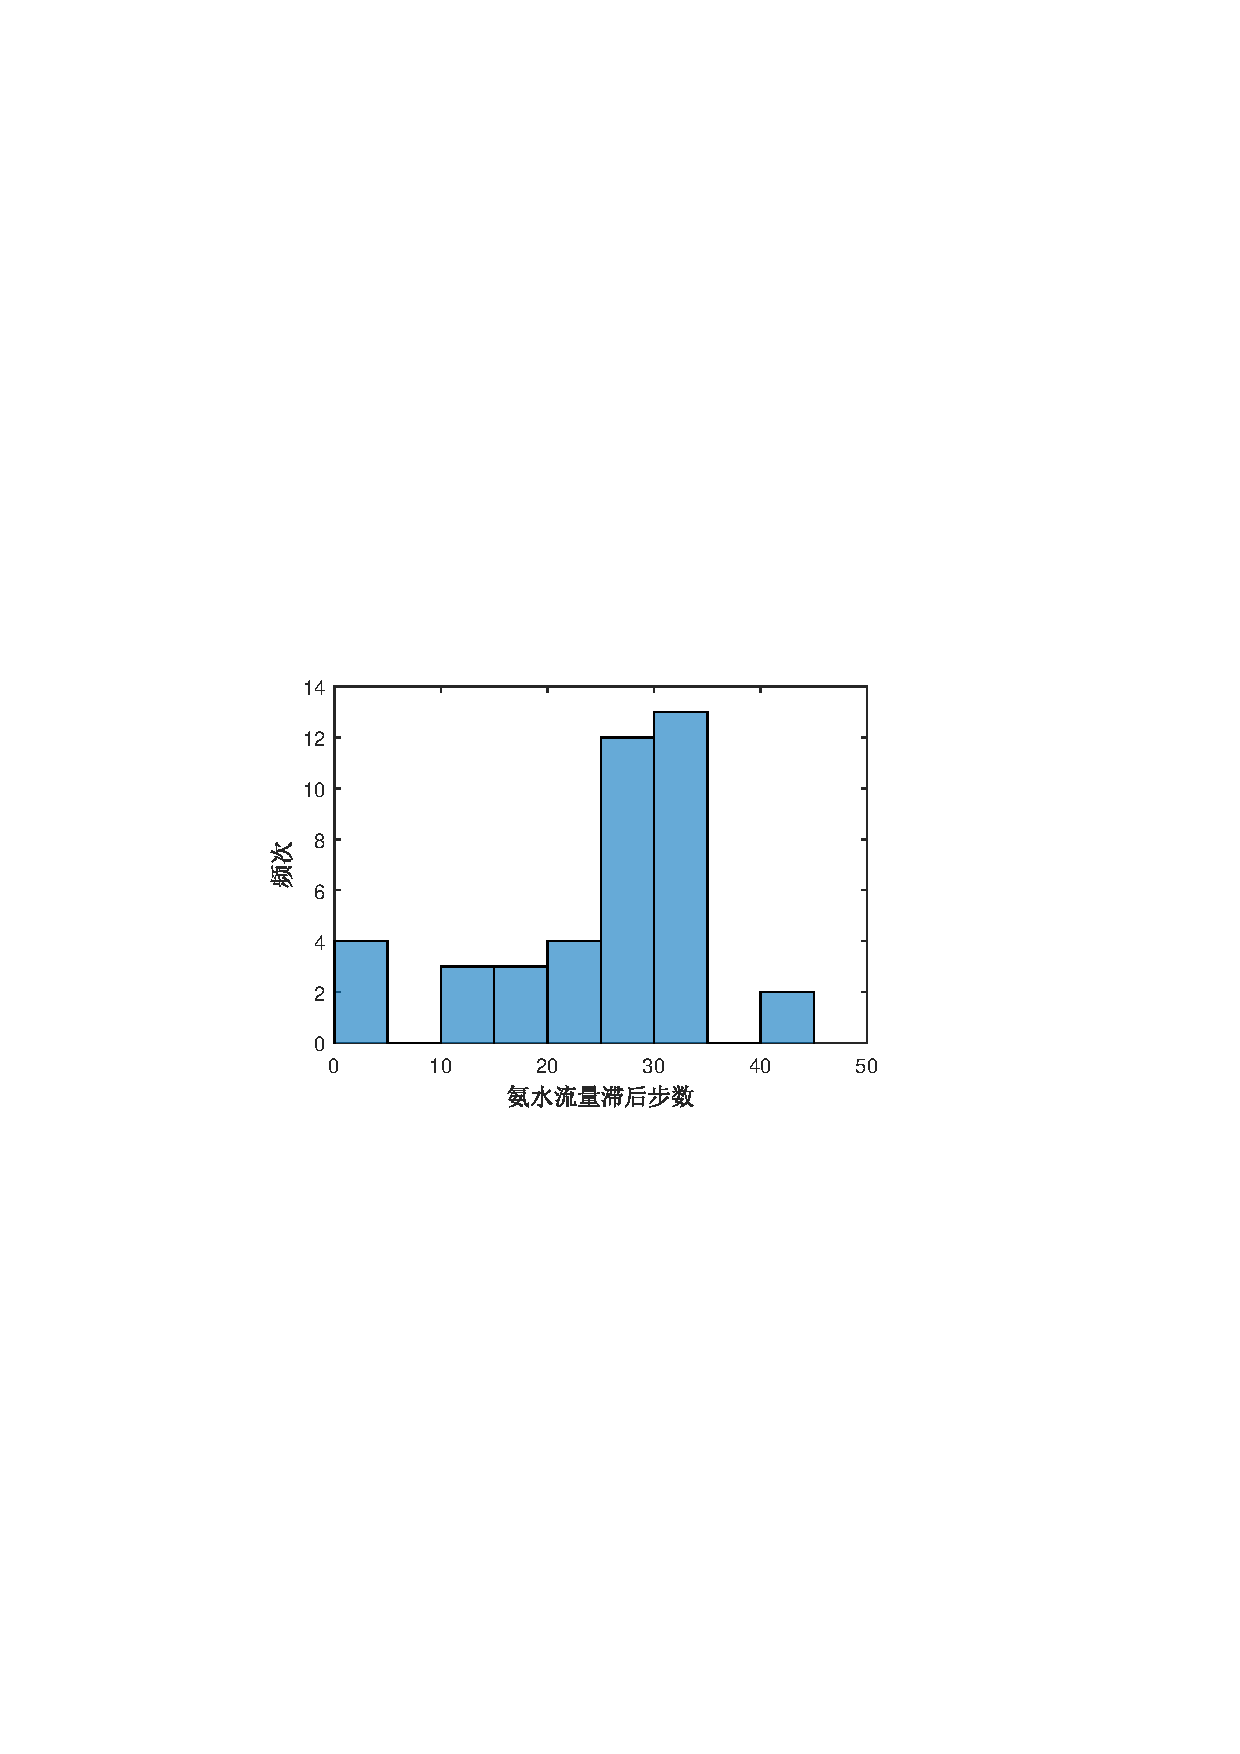
\includegraphics{delay_hist}
\caption{氨水流量滞后步数直方图} \label{fig:delay_hist}
\end{figure}
\section{基于多元线性回归的氮氧化物软测量}
\subsection{多元线性回归}
多元线性回归模型如式~\ref{equ:reg}~所示,式中$x_{i}$为第$i$个模型输入,$y$为~\ce{NOx}排放值,$q$为模型输入集基数, $\beta_{0}$为线性模型截距项。
\begin{equation}
\label{equ:reg}
y= \beta_{0}+\sum_{j=1}^{q}{\beta_{j}}{x_{j}}+\varepsilon
\end{equation} 

参照最小二乘准则的定义,给出式~\ref{equ:tar_reg}~所示的目标函数
\begin{equation}
\label{equ:tar_reg}
{S}(\bm{\beta})=\sum_{i=1}^{n}{\varepsilon_{i}^{2}}=(\bm{Y}-\bm{X}\bm{\beta})^{T}(\bm{Y}-\bm{X}\bm{\beta})
\end{equation}
其中$\bm{\beta} = {\begin{pmatrix} \beta_{1} & \beta_{2} &\cdots & \beta_{q} \end{pmatrix}}^{T}$,$\bm{Y} = {\begin{pmatrix} Y(1) & Y(2) &\cdots & Y(n) \end{pmatrix}}^{T}$,

\noindent
$\bm{X} = \left[{\begin{array}{ccccc}
1&x_{1}{(1)}  & x_{2}{(1)}&\cdots&x_{q}{(1)}\\
1&x_{1}{(2)}  & x_{2}{(2)}&\cdots&x_{q}{(2)}\\
\vdots & \vdots  &\vdots &\ddots  &\vdots\\
1&x_{1}{(n)}  & x_{2}{(n)}&\cdots&x_{q}{(n)}
\end{array}}\right]$
   
由批处理最小二乘估计得待估计量为
\begin{equation}
{\bm{\hat{\beta}}}=(\bm{X}^{T}\bm{X})^{-1}\bm{X}^{T}\bm{Y}
\end{equation}

\subsection{自变量选择方法}

在多元回归分析中,回归变量的选择对回归方程的质量有重要的影响。若遗漏了重要的回归变量,回归模型的效果不会好;若引入过多的回归变量,则可能出现过拟合,影响模型的稳定性。回归变量选择的方法主要有四种:最优子集法、向后剔除法、向前选择法、逐步回归法。

最优子集法考虑输入变量集合的所有子集,找出其中的最优子集作为模型输入。对于含有$q$个候选输入变量的模型,其输入变量子集有$2^{q}$个。随着$q$ 的增大,逐个尝试找出最优子集模型的计算代价指数上升。此外,最优子集法选出的模型只是对训练段拟合最好的模型,对测试数据段不一定适用。对~\ce{NOx}~模型来说,其候选输入变量有10个,候选子集有1024个,逐一找出最优子集是比较耗时耗力的。另外,这里的最优子集也只是对训练数据段的最优子集,不能保证其在测试数据段的性能优于其它子集模型。

其余三种方法都属于逐步型程序,其计算复杂度相对最优子集法来说很小,特别适用于候选变量较多的情况。向后剔除方法首先建立含有全部回归变量的模型,逐步从模型中剔除回归变量来计算最优子集,知道剩余的变量不能被剔除。向前选择法从不含回归变量的模型开始,通过逐步向模型中加入回归变量来尝试求解最优子集。逐步回归法结合了向前选择和向后剔除,在逐步加入回归变量的过程中利用信息准则进行检验,若没有通过检验则采用向后剔除法,两种方法交替进行直到找到所有的显著变量,且选择的所有变量都是显著的\cite{montgomery2015introduction}。

比较回归模型质量需要有相应的性能指标,也称作信息准则。用于回归变量选择的信息准则主要有F检验、MSE(Mean Square Error,均方误差)、$\textrm{R}^{\textrm{2}}$、调整的$\textrm{R}^{\textrm{2}}$、Mallows $\textrm{C}_{\textrm{p}}$、AIC(Akaike Information Criterion,赤池信息准则)、BIC(Bayesian Information Criterion,贝叶斯信息准则)等等。其中,AIC和BIC是两种最具代表性的信息准则\cite{yong2005can}。相比单纯使用拟合程度来衡量模型质量的信息准则,AIC和BIC都增加了对模型使用的变量个数的考虑,要求模型尽可能用较少的变量解释回归量的变化,能够有效地防止过拟合,使模型具有较高地预测能力。因此,本文基于AIC、BIC两种信息准则,采用向前选择法、向后剔除法、逐步回归法三种方法来选择输入变量,并比较其性能差异。这两种信息准则的值越小,代表模型的质量越高。

AIC准则如式~\ref{equ:aic_normal}~所示,在最小二乘回归中可由式~\ref{equ:aic_ls}~计算
\begin{align}
AIC &= -2\ln (L) + 2p \label{equ:aic_normal}\\
AIC &= n\ln(\frac{SS_{Res}}{n})+2p \label{equ:aic_ls}
\end{align}

Schwartz提出的BIC准则如式~\ref{equ:bic_normal},在最小二乘回归下可由式~\ref{equ:bic_ls}~计算。
\begin{align}
BIC &= -2\ln (L) + p\ln(n) \label{equ:bic_normal}\\
BIC &= n\ln(\frac{SS_{Res}}{n})+p\ln(n) \label{equ:bic_ls}
\end{align}
其中$L$为似然函数,$p$是模型中的变量个数, $SS_{Res} = \sum_{i=1}^{n}(y_{i} - \hat{y}_{i})$。 
\subsection{静态软测量模型}
\label{chap:static_model}

选择某三天的数据,前$L_{m}$个点作为训练段数据建立静态软测量模型,其余数据作为测试段数据。表~\ref{tab:input_not_select}~给出了几组不同$L_{m}$下不同变量选择方法未选择的自变量,不同序号代表不同的回归变量,其具体含义见表~\ref{tab:nox_input}。为了方便起见,back代表后向选择,forward代表前向选择,both代表逐步回归。这里后向选择法从含有全部10个变量的模型开始,前向选择和逐步回归均从不含任何变量的模型开始,直到选出让信息准则极小的全部回归变量。
\begingroup
\renewcommand*{\arraystretch}{1.67}
\begin{table}[!h]
\small
\centering
\caption[未被选中的模型输入量]{未被选中的模型输入量} \label{tab:input_not_select}
\begin{tabular}{ccccccc}
\hline\hline 
$L_{m}$&	AIC back	&AIC forward	&AIC both	&BIC back	&BIC forward&	BIC both\\
\hline
1000	&1	&1&	1	&1 6 8 9	&1 6 8 9	&1 6 8 9\\
2000	&8	&7&	8	&8&	4 7	&4 7\\
3000	&8	&-	&8	&8	&7 10	&7 10\\
4000	&4	&4 8	&4 8	&3 7 10	&4 8 10	&4 8 10\\
5000	&2 4	&4	&2 4	&2 4	&4 7	&4 7\\
\hline\hline
\end{tabular}
\end{table}
\endgroup

由表~\ref{tab:input_not_select}~可看出,利用不同的建模数据,选出来的模型输入量是不同的;采用不同的信息准则,选出的自变量也不一样;即使采用同一种信息准则,不同的变量选择方向也会导致选出的结果不同。

选择的自变量不同,就意味着模型在测试段性能存在一定差异。选用MaxAE(Maximum Absolute Error,最大绝对误差)和RMSE(Root Mean Square Error,均方根误差)作为模型的性能指标。在实际建模过程中,建模所用数据长度$L_{m}$的选择具有相当大的随意性。因此,有必要研究在$L_{m}$变化的情况下,是否会有一种变量选择方法优于其他方法。采用网格搜索法,研究$L_{m}$为$\{\textrm{50},\,\textrm{100},\,\textrm{150},\cdots,\textrm{5000}\}$时,不同自变量选择方法获得的模型性能。

以AIC双向选择和BIC双向选择为例,图~\ref{fig:diff_lm_mae_rmse}~分别给出模型在不同$\textrm{L}_{\textrm{m}}$处的最大误差和均方根误差。由于个别点处误差过大,在不影响定性结论的前提下,对其限幅。
\begin{figure}[!hbt]
\centering
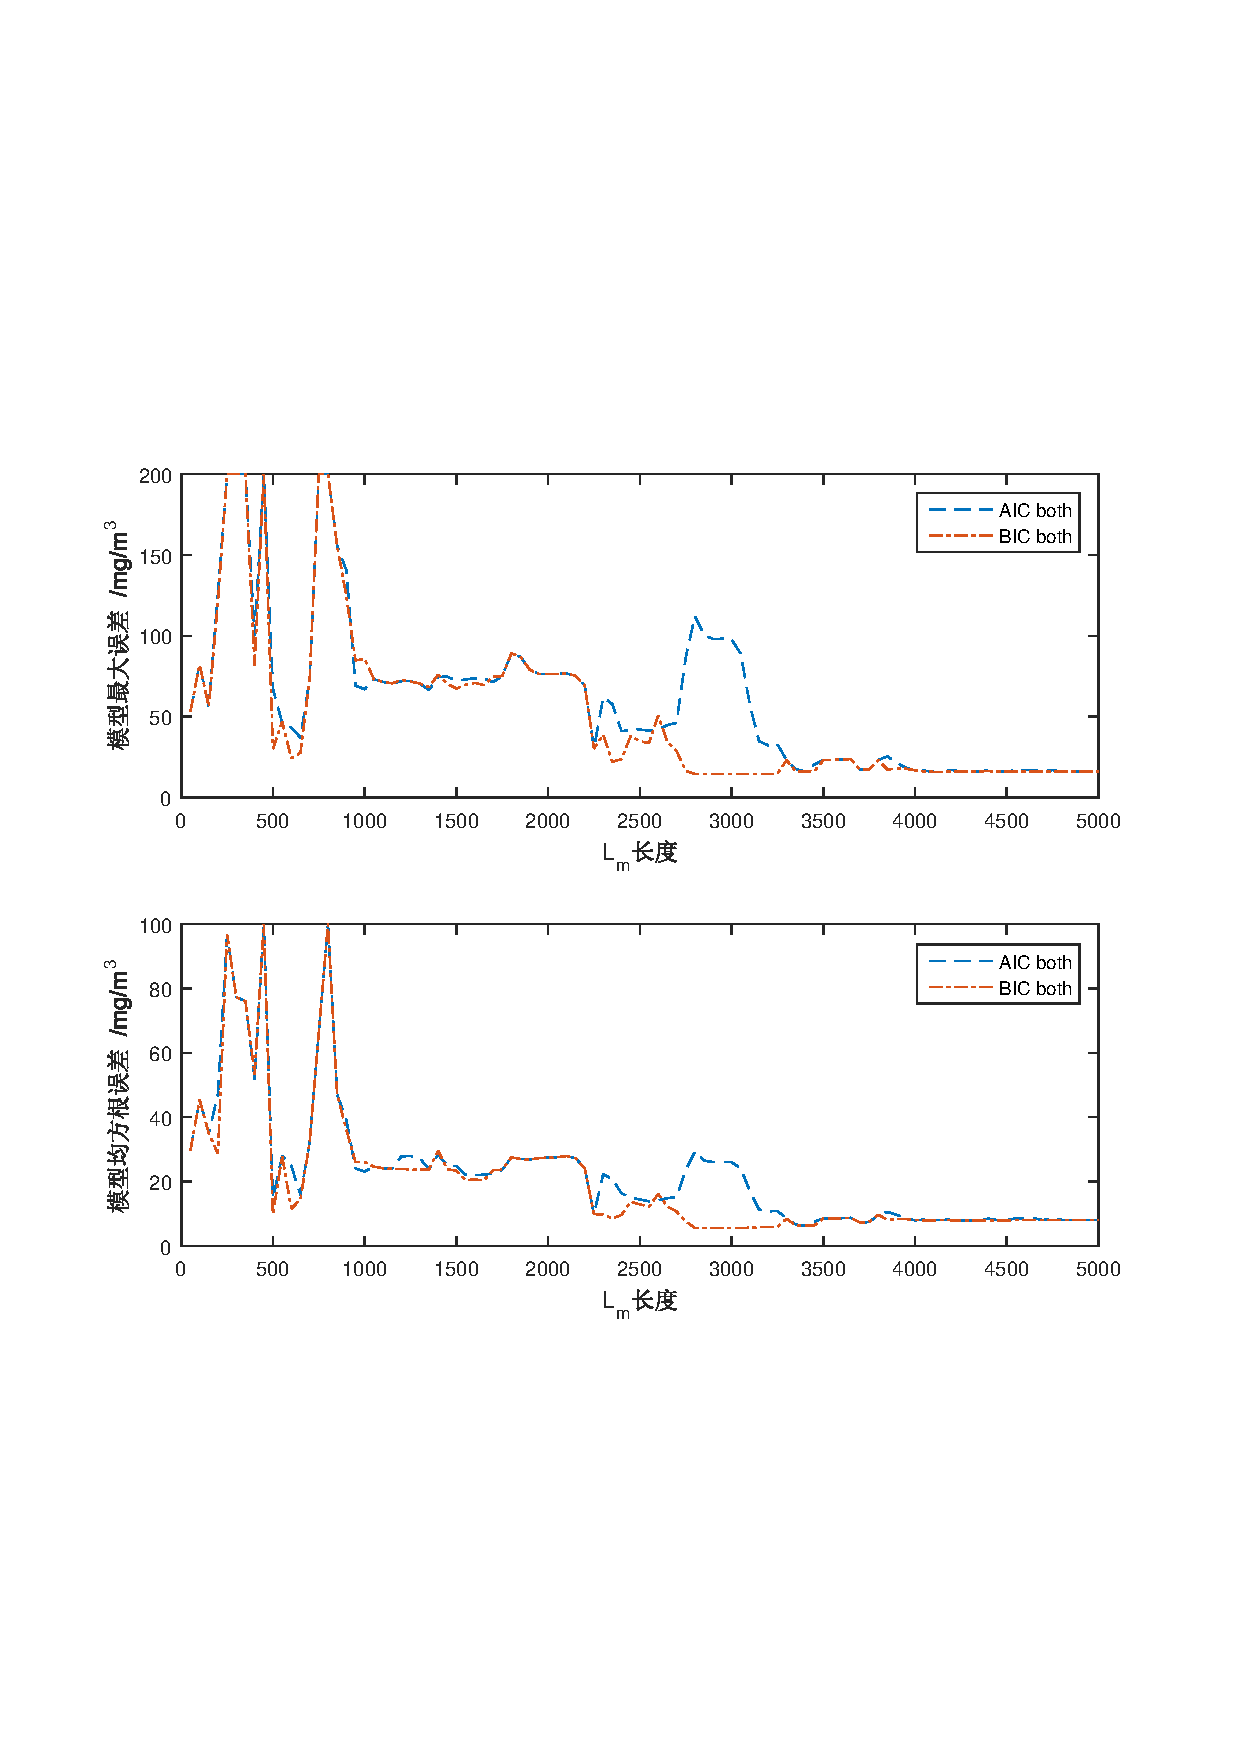
\includegraphics[width=13cm]{diff_lm_mae_rmse}
\caption{双向选择模型最大误差和均方根误差} \label{fig:diff_lm_mae_rmse}
\end{figure}

可以看出,当建模所用数据量较少(少于1000个数据点)时,两种变量选择方法得到的模型性能与采用数据点个数都没有表现出明显的关系。只有在个别取值附近,模型的误差才比较小。$L_{m}$在$[\textrm{1000},\,\textrm{2300}]$内变化时,模型性能基本没有太大变化。$L_{m}$大于2300后,基于BIC双向选择法的模型误差一直处于较低的水平,模型误差在$L_{m}$等于3000附近时达到谷底,其后随${L}_{m}$增大,模型误差反而略有上升。基于AIC双向选择法的模型误差在$[\textrm{2500},\,\textrm{3500}]$段振荡,随后达到与BIC相近的水平。最后模型最大误差基本稳定在20$\,$\si{mg/m^3}附近,均方根误差稳定在7$\,$\si{mg/m^3}附近。

现场~\ce{NOx}~的测量范围为0-300$\,$\si{mg/m^3},参考~\ce{NOx}~测量仪表,规定如下两个软测量模型误差幅值要求:现场量程最大值为300$\,$\si{mg/m^3},模型最大误差小于量程的10$\,$\si{\percent},即30$\,$\si{mg/m^3};现场测量值一般在100$\,$\si{mg/m^3}以下,均方根误差应小于测量值的10$\,$\si{\percent},取9$\,$\si{mg/m^3}。当$L_{m}$取$\{\textrm{50},\,\textrm{100},\,\textrm{150},\cdots,\textrm{5000}\}$,不同自变量选择方法得到的满足性能要求的模型个数不同,见表~\ref{tab:static_model_percent}~。基于AIC信息准则选择自变量时,三种不同的选择方向得到的结果相差不多。基于BIC信息准则的变量选择方法时,双向选择最好,后向选择最差。基于BIC信息准则选出了更多满足要求的模型。
\begingroup
\renewcommand*{\arraystretch}{1.67}
\begin{table}[!h]
\small
\centering
\caption[满足误差幅值要求的静态软测量模型百分比]{满足误差幅值要求的静态软测量模型百分比} \label{tab:static_model_percent}
\begin{tabular}{ccccccc}
\hline\hline 
	&AIC back	&AIC forward	&AIC both	&BIC back	&BIC forward	&BIC both\\
\hline
MaxAE<30	&35	&35	&35	&39	&49	&51\\
RMSE<9	&32	&31	&32	&35	&44	&46\\
两个都满足	&32	&31	&32	&35	&44	&46\\
\hline\hline
\end{tabular}
\end{table}
\endgroup

\begin{figure}[!hbt]
\centering
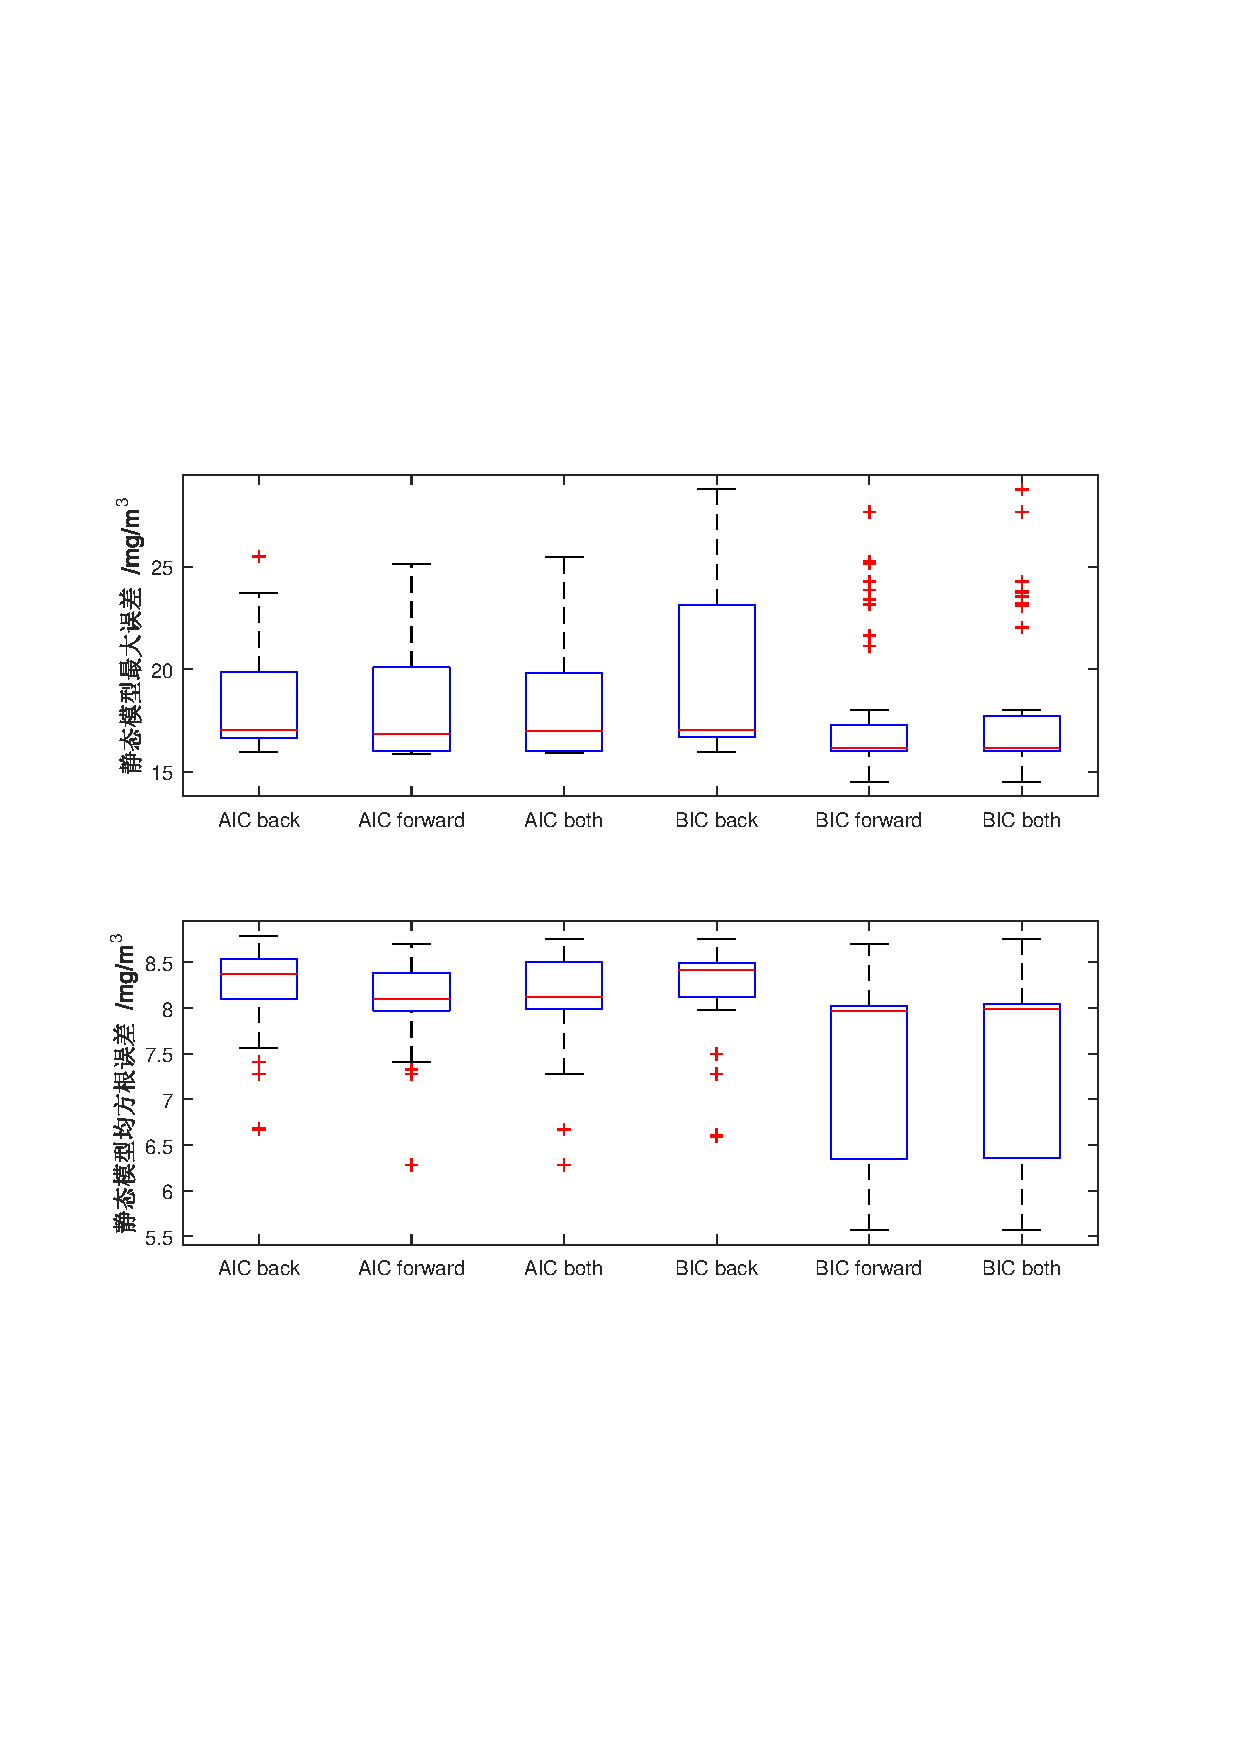
\includegraphics[width=13cm]{static_model_boxplot}
\caption{静态模型最大误差、均方根误差箱线图} \label{fig:static_model_boxplot}
\end{figure}

实际上,不同变量选择方法结果的最大误差和均方误差的数据分布特征也是不同的。图~\ref{fig:static_model_boxplot}~中分别给出了满足MaxAE和RMSE的静态模型误差箱线图。可以看出,基于AIC准则的模型大部分最大误差都分布在$[\textrm{16},\,\textrm{20}]$,大部分均方根误差分布在$[\textrm{7.5},\,\textrm{9}]$,个别模型的均方根误差在$[\textrm{6},\,\textrm{7.5}]$。基于BIC后向选择方法的模型表现最差。基于BIC的前向选择和双向选择得到了更低的MaxAE和RMSE下限,其MaxAE和RMSE的第三四分位数明显低于其它方法。即使同样满足误差幅值的要求,基于BIC的前向选择或双向选择得到的模型性能也要优于其它几种方法。

\section{结合滚动窗的软测量模型}
\subsection{结合滚动窗的线性回归算法}

实际系统的状态只与当前工作点附近的数据有较大相关性,而与远离工作点附近的数据相关性不大。工业过程由于进料、温度、工艺等因素的变化,工作点往往会发生迁移。因此,采用固定数据得到的模型难以保证模型的准确性。滚动窗方法建立随时间滚动的建模数据区间,在每个新的数据到来时都会更新模型,从而保证模型始终反映系统当前状况。但对于流程工业来说,这种频繁的模型更新会给控制系统带来较大的计算负担,且在系统工作点没有发生较大变化时,频繁更新模型往往是不必要的。因此,在滚动窗方法中引入模型更新周期,模型只有在达到更新周期时才进行更新,这样既可以保证模型的准确性,又可以降低控制系统的计算量。
记$T_{s}$为系统的采样周期,$T_{u}$为模型更新周期,$L_{s} = T_{u}/T_{s}$ 为窗口滚动距离,滚动窗窗口长度即为建模所用数据长度$L_{m}$。随着系统运行,旧的数据移出窗口,新的数据进入窗口,当达到模型更新周期时,模型更新。

基于滚动窗的多元回归建模步骤如下:
\begin{enumerate}
\item {设置窗口长度$L_{m}$和模型滚动距离$L_{s}$;} 
\item {选择窗口样本数据,数据预处理;}
\item {利用窗口数据基于多元线性回归方法建模;}
\item{预测~\ce{NOx}~排放量;}
\item{有新的~\ce{NOx}~测量数据时,基于数据预处理方法判断该测量值是否为异常值。是则转6,否则转7;}
\item{异常测量值置为相应~\ce{NOx}~预测值;}
\item{利用新的测量数据更新更新窗口样本;}
\item {是否达到模型更新周期,是则转3,否则转4。}
\end{enumerate}

\subsection{窗口长度和滚动距离对模型的影响}

取$L_{m}$为$\{\textrm{50},\,\textrm{100},\,\textrm{150},\cdots,\textrm{5000}\}$,$L_{s}$为$\{\textrm{20},\,\textrm{40},\,\textrm{60},\cdots,\textrm{2000}\}$,共计10000种参数组合,仍采用~\ref{chap:static_model}~节中的两个误差幅值要求,研究滚动窗参数对软测量模型的影响。
图给出了不同$L_{m}$长度下,采用不同变量选择方法得到的满足MaxAE幅值要求的滚动窗软测量模型。在$L_{m}$较小时,即使结合滚动窗方法,也很少有模型满足MaxAE的要求。随$L_{m}$增大,AIC前向选择方法的百分比上升速度最快。在$L_{m}$大于3500后,几乎所有的变量选择方法都有超过90$\,\%$的模型满足要求。

\begin{figure}[!hbt]
\centering
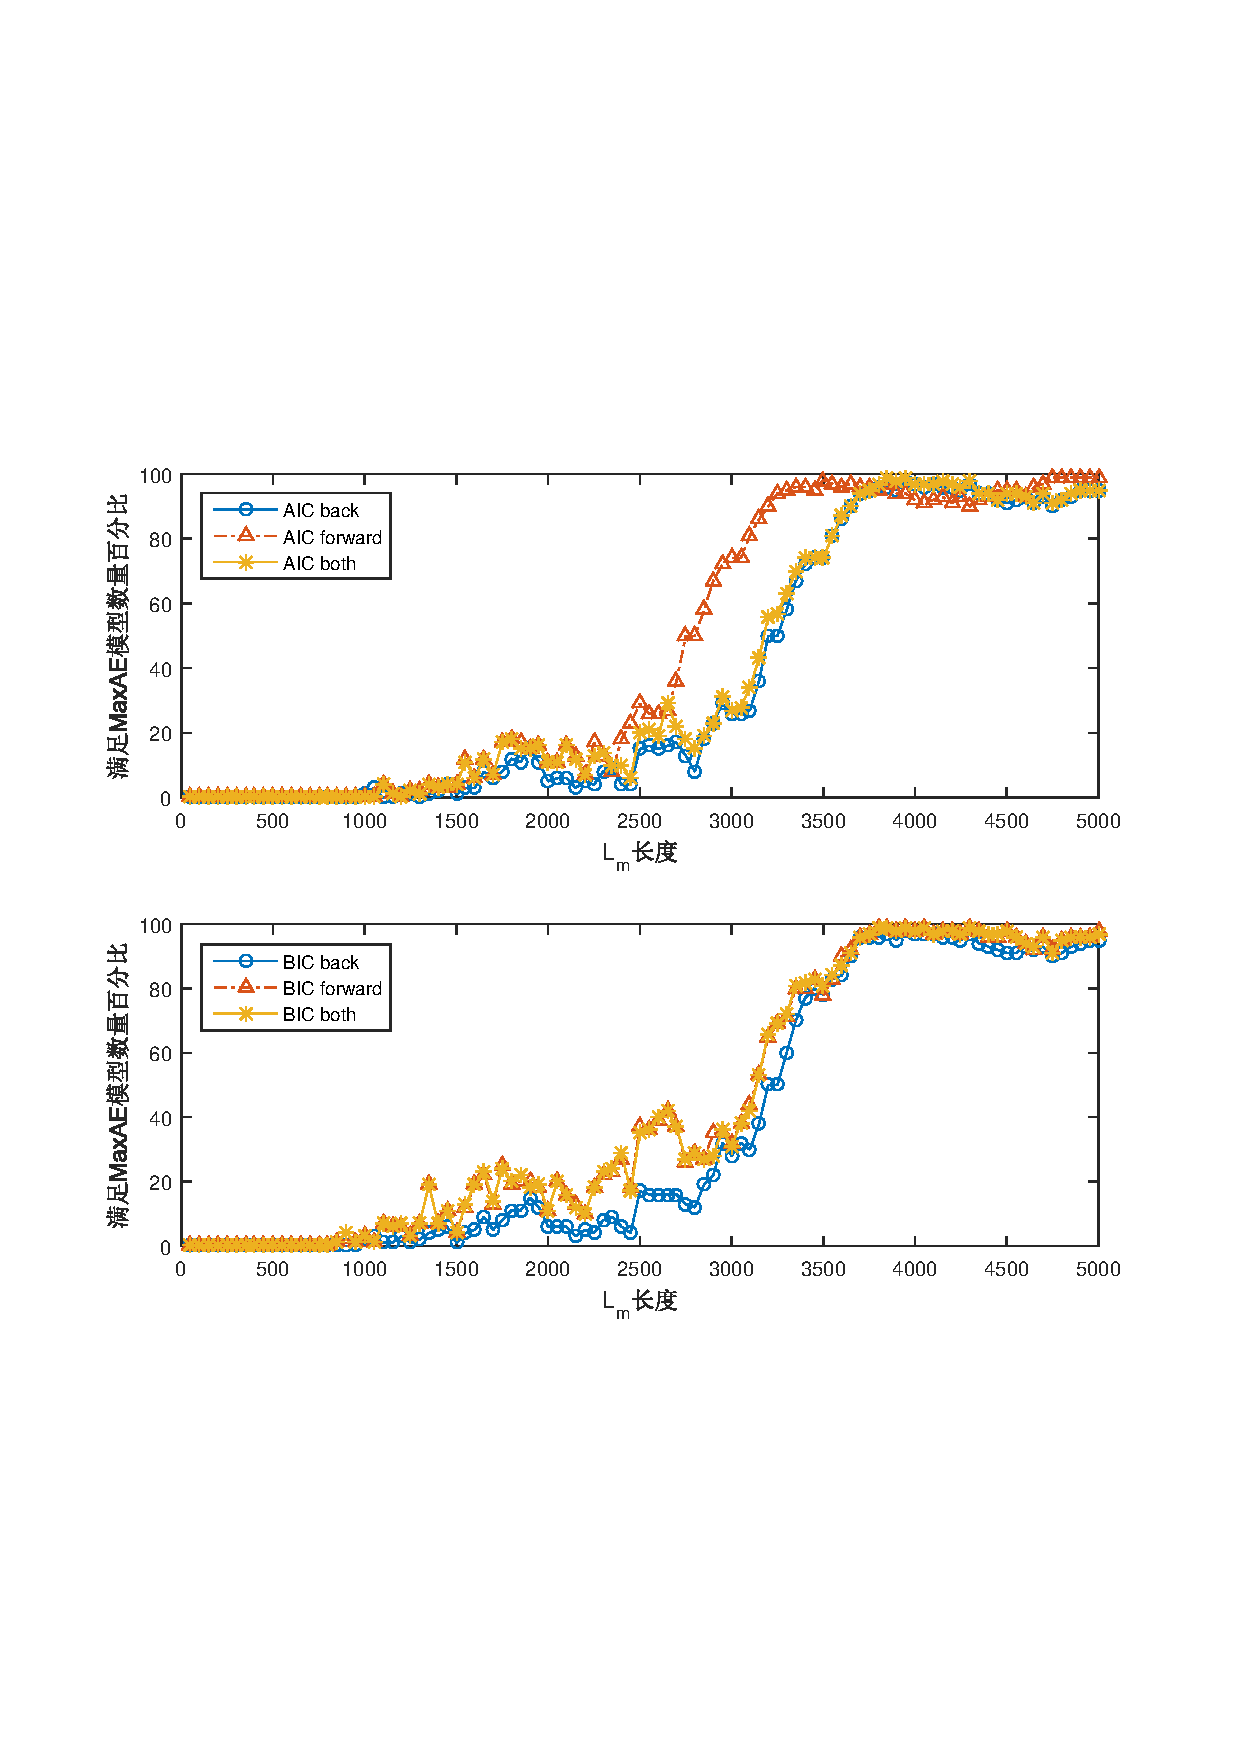
\includegraphics[width=13cm]{diff_lm_model_num_mae}
\caption{满足MaxAE要求的模型数量百分比1} \label{fig:diff_lm_model_num_mae}
\end{figure}
 
 \begin{figure}[!hbt]
\centering
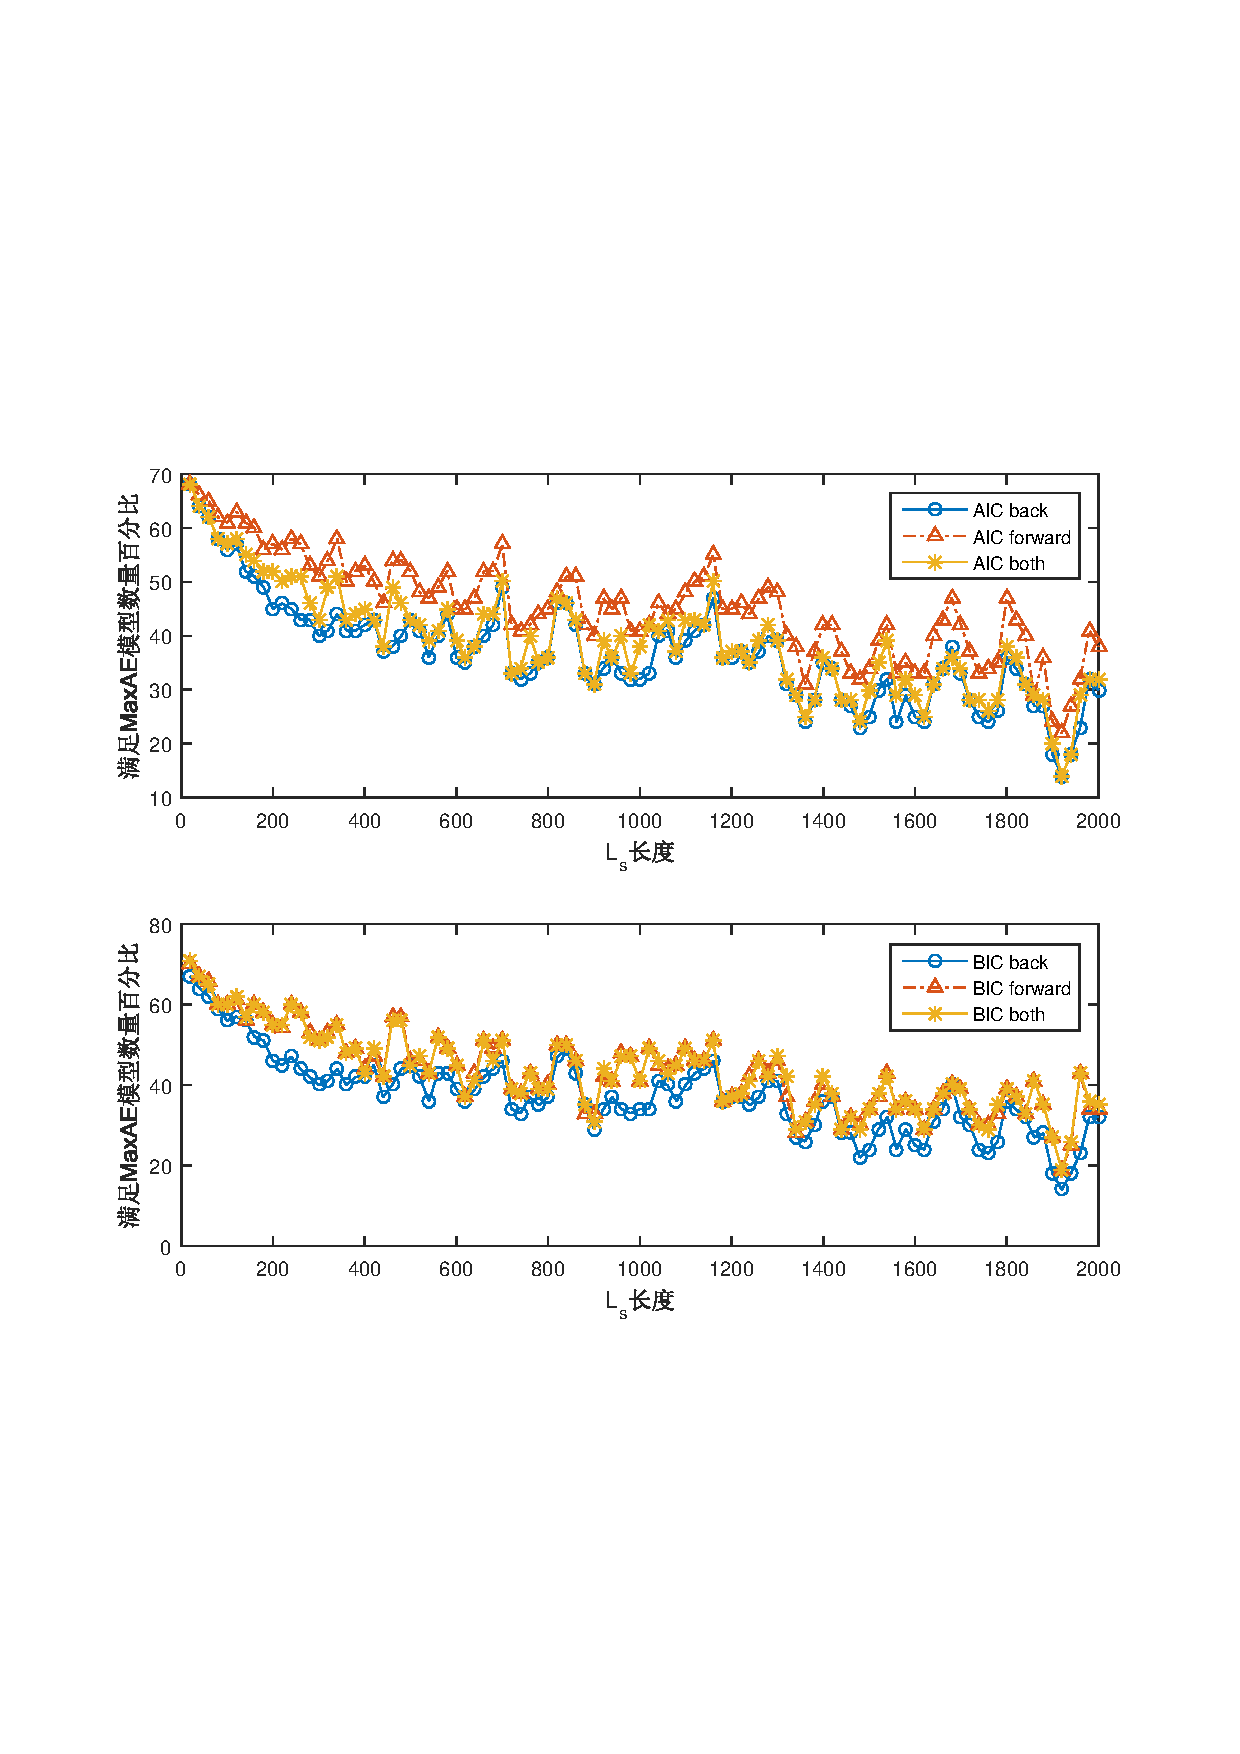
\includegraphics[width=13cm]{diff_ls_model_num_mae}
\caption{满足MaxAE要求的模型数量百分比2} \label{fig:diff_ls_model_num_mae}
\end{figure}

\begin{figure}[!hbt]
\centering
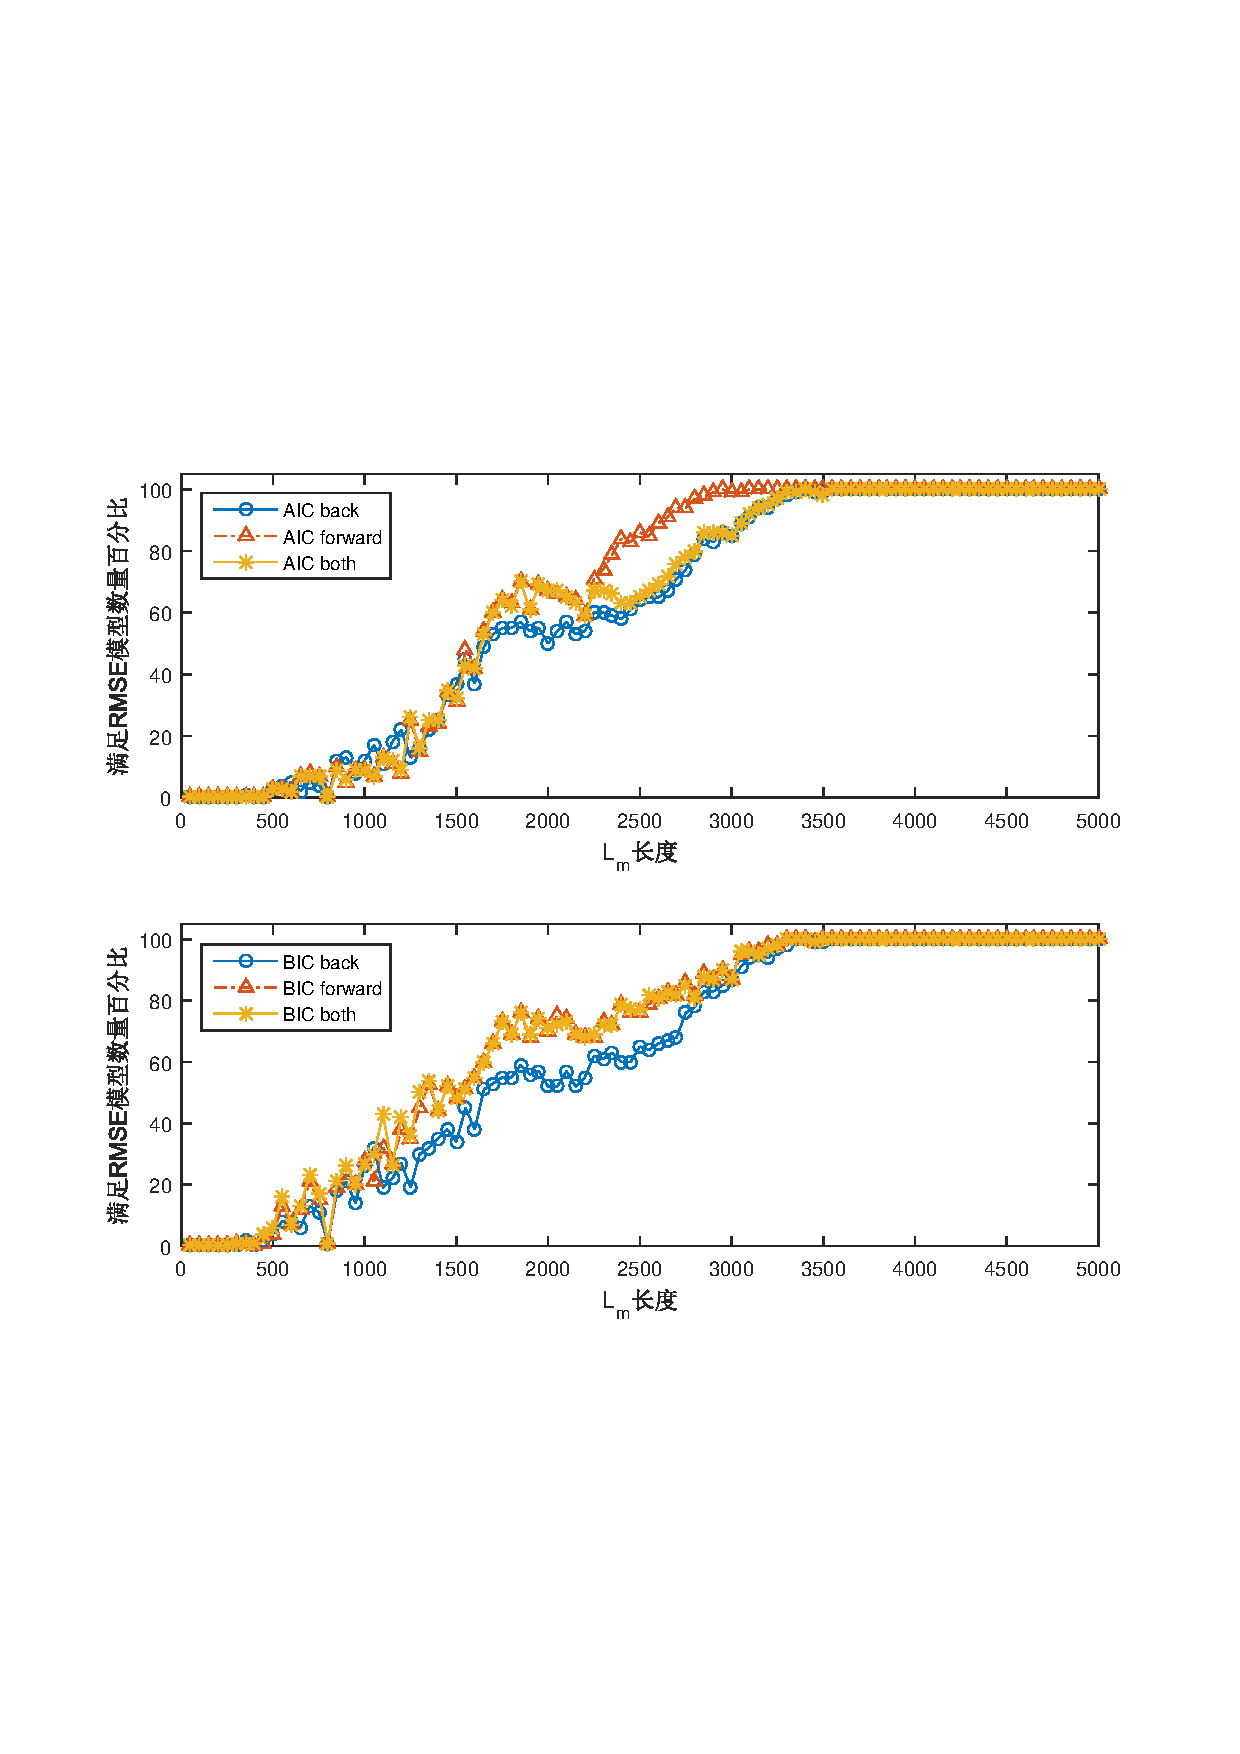
\includegraphics[width=13cm]{diff_lm_model_num_rmse}
\caption{满足RMSE要求的模型数量百分比1} \label{fig:diff_lm_model_num_rmse}
\end{figure}

\begin{figure}[!hbt]
\centering
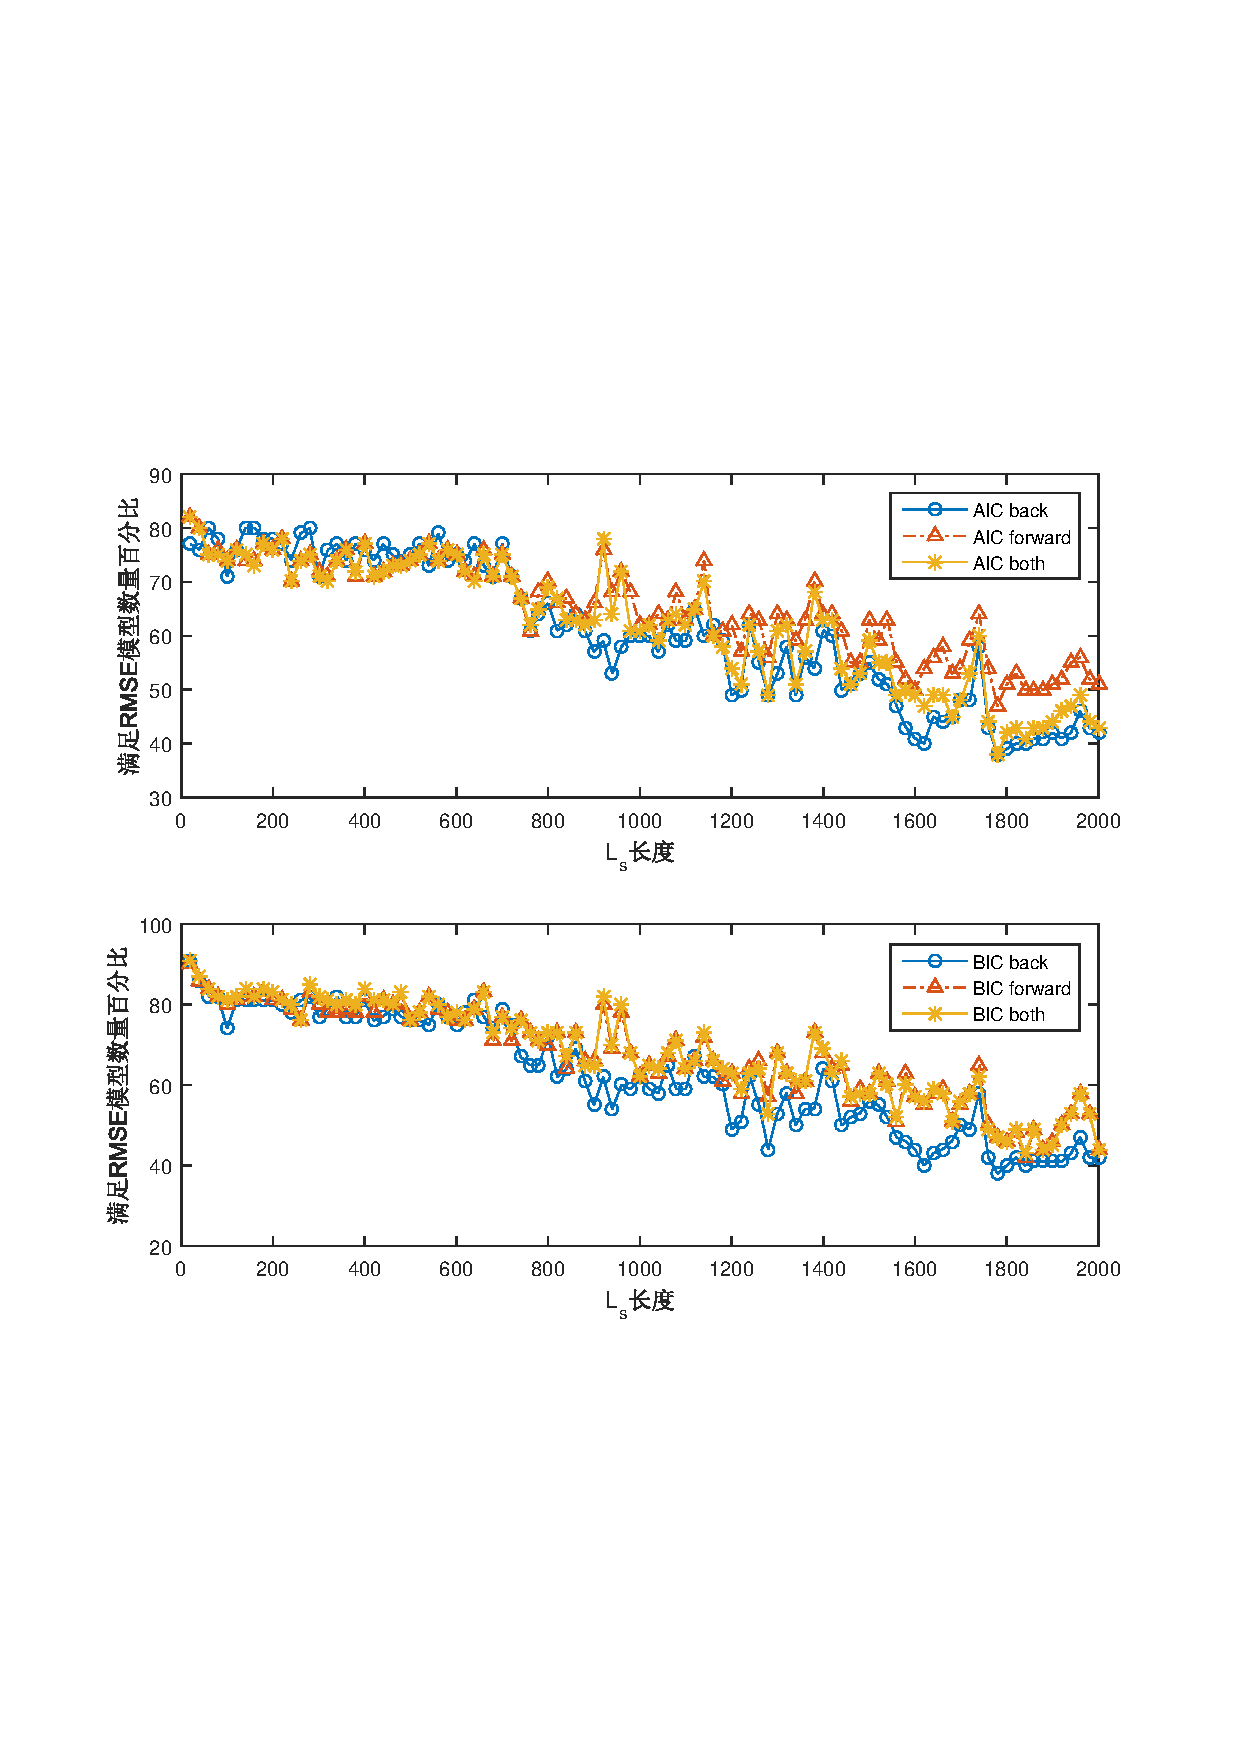
\includegraphics[width=13cm]{diff_ls_model_num_rmse}
\caption{满足RMSE要求的模型数量百分比2} \label{fig:diff_ls_model_num_rmse}
\end{figure}
   
图~\ref{fig:diff_ls_model_num_mae}~为不同$L_{s}$对应的满足MaxAE要求的模型数量百分比。随$L_{s}$增大,满足MaxAE要求的模型占比逐渐降低,过程虽然有波动,但始终没有超过$L_{s}$小于200时的比例。另外,在大部分区间内,后向选择方法的选择效果要比其它两种选择方法差。

图~\ref{fig:diff_lm_model_num_rmse}、\ref{fig:diff_ls_model_num_rmse}~分别给出随$L_{m}$、$L_{s}$变化,满足RMSE要求的模型数量百分比。随着$L_{m}$增大,满足RMSE要求的模型百分比很快开始上升,同样$L_{m}$在约为3500后趋向于稳定。随$L_{s}$上升,满足RMSE要求的模型百分比先保持平稳,$L_{s}$大于700后才开始下滑,即使$L_{s}$到达2000,也有30$\,$\si{\percent}的模型满足RMSE指标。


因此,选择$L_{m}$时要取一个稍大的值,虽然这会使得建模需要的计算量增加,但也会使得更多的模型满足RMSE和MaxSE指标。$L_{s}$可以取一个适中的值,降低因$L_{m}$取值偏大增加的计算量,又保障系统的性能。
\begingroup
\renewcommand*{\arraystretch}{1.67}
\begin{table}[!h]
\small
\centering
\caption[满足误差幅值要求的滚动窗软测量模型百分比]{满足误差幅值要求的滚动窗软测量模型百分比} \label{tab:sw_model_percent}
\begin{tabular}{ccccccc}
\hline\hline 
	&AIC back	&AIC forward	&AIC both	&BIC back	&BIC forward	&BIC both\\
\hline
MaxAE<30	&36.80&45.54	&38.95	&37.45	&43.38	&43.44\\
RMSE<9	&60.92	&65.28&	62.45	&62.54	&67.87	&68.28\\
两个都满足	&36.80&	45.54	&38.95	&37.45	&43.38	&43.44\\
\hline\hline
\end{tabular}
\end{table}
\endgroup

表~\ref{tab:sw_model_percent}~中给出了满足~\ref{chap:static_model}~节中误差幅值要求的滚动窗模型比例。对比表 \ref{tab:static_model_percent} 可以看出,不论采用哪种变量选择方法,满足均方根误差的模型比例都提高了不少。但是,对于BIC选择方法来说,满足最大误差要求的最大模型百分比却下降了,即使是AIC选择,满足最大误差要求的模型百分比也没有特别明显的提高。

\begin{figure}[!hbt]
\centering
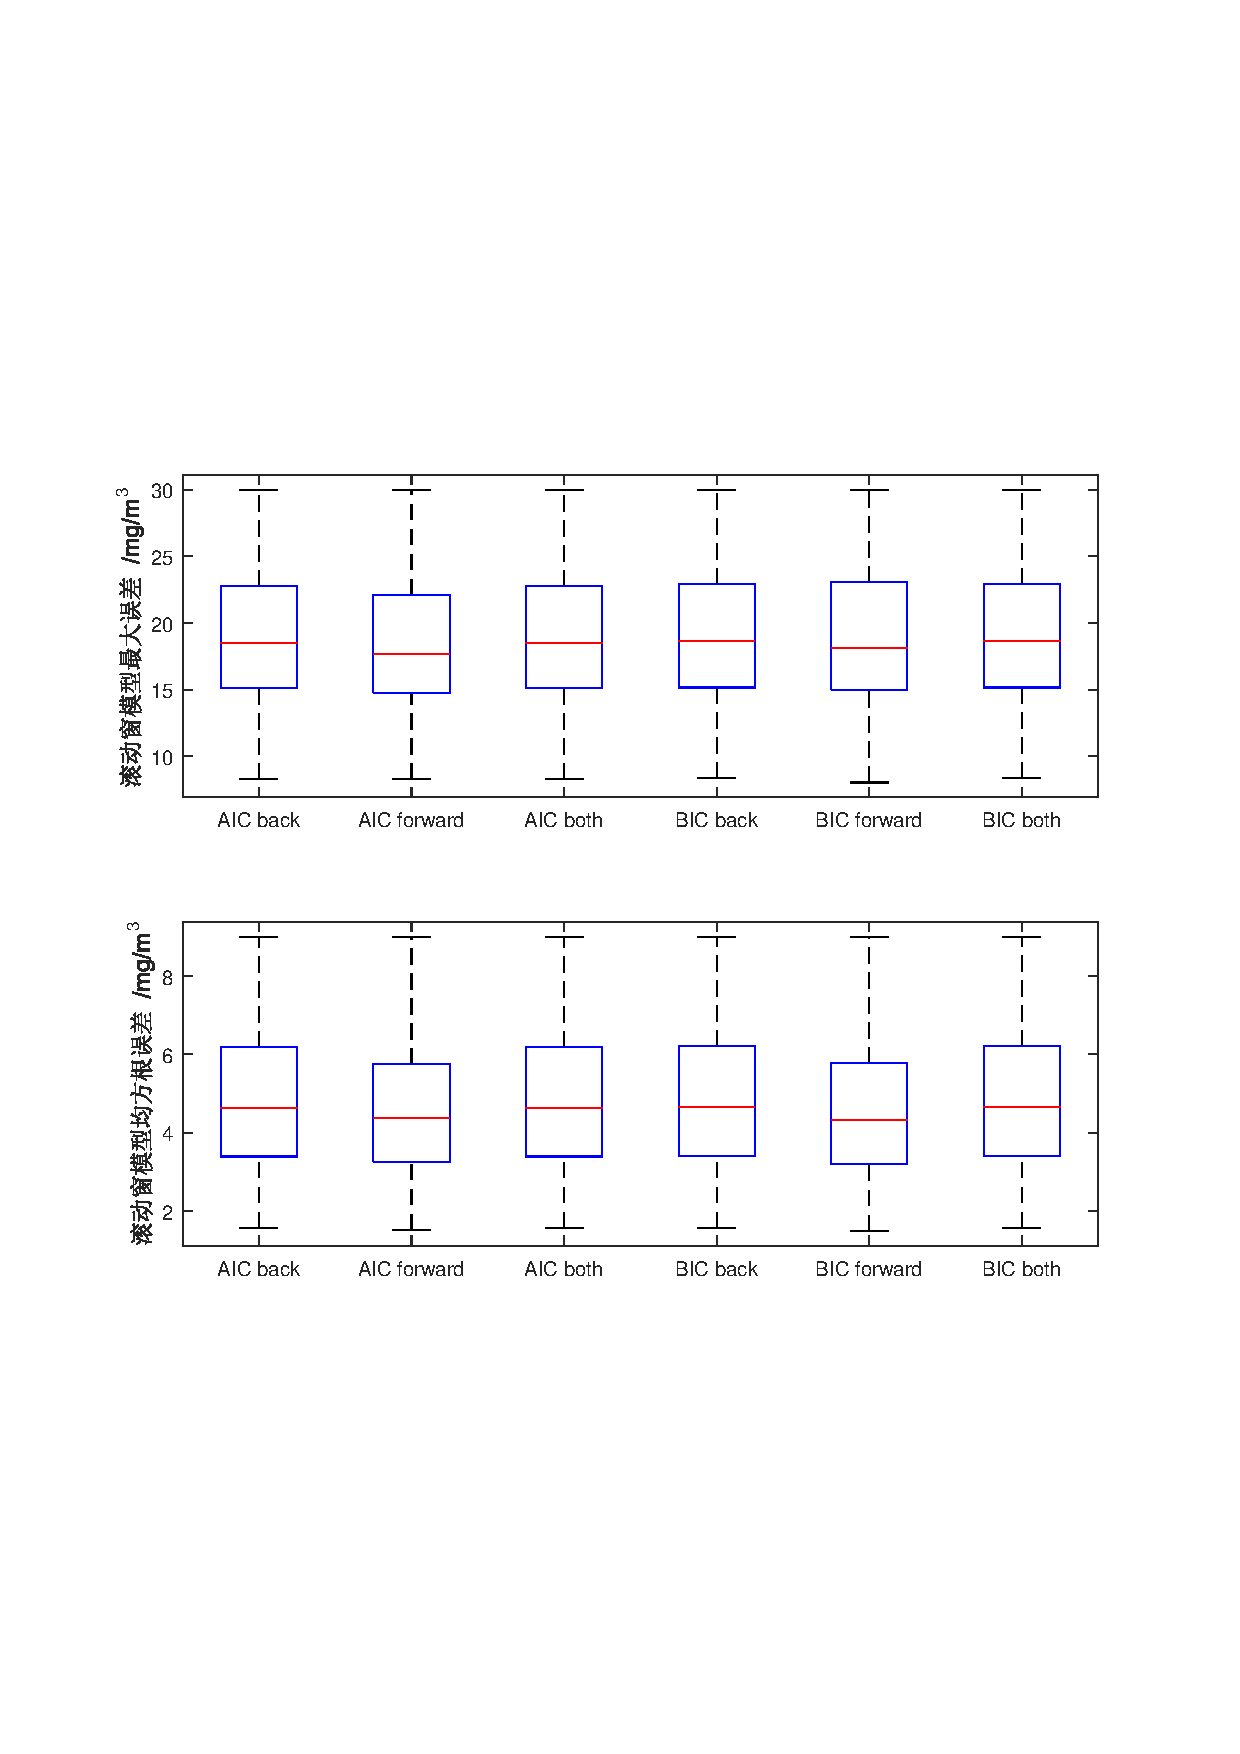
\includegraphics[width=13cm]{slide_model_boxplot}
\caption{滚动窗模型最大误差、均方根误差箱线图} \label{fig:slide_model_boxplot}
\end{figure}

图~\ref{fig:slide_model_boxplot}~为满足MaxAE和RMSE指标的滚动窗模型误差箱线图。其中AIC前向选择模型的误差中位数低于其它方法,各种方法达到的MaxAE和RMSE下限水平基本相当,最大误差下限约为9$\,$\si{mg/m^3},均方根误差下限约为1.75$\,$\si{mg/m^3}。对比图~\ref{fig:static_model_boxplot}~可以发现,采用滚动窗思想建立的软测量模型的最大误差下限有所下降,但就中位值而言变化不大;均方根误差达到了更低的下界,且中位值和第三四分位数也有明显降低。这说明结合滚动窗的软测量方法能够显著降低模型的均方根误差,而且对模型的最大误差也有一定的抑制作用。

\subsection{结合滚动窗的软测量模型预测效果}
图~\ref{fig:soft_sensor_res}~给出了结合滚动窗方法采用BIC双向选择的软测量模型的预测结果,这里$L_m$取5000,$L_s$取30,软测量模型每5$\,$\si{\min}更新一次,模型运行48$\,$\si{\hour}。其中,69.54$\,\%$的预测值与实际测量值偏差不超过1.5$\,$\si{mg/m^3},97.58$\,\%$的预测值与实际测量值偏差不超过4.5$\,$\si{mg/m^3},99.87$\,\%$的预测值与实际测量值偏差不超过9$\,$\si{mg/m^3},最大偏差为11.78$\,$\si{mg/m^3},均方根误差为1.760$\,$\si{mg/m^3}。即使在工况发生较大变化的情况下,软测量模型也能够比较快地跟踪工况变化,保持较好的预测效果。
\begin{figure}[!hbt]
\centering
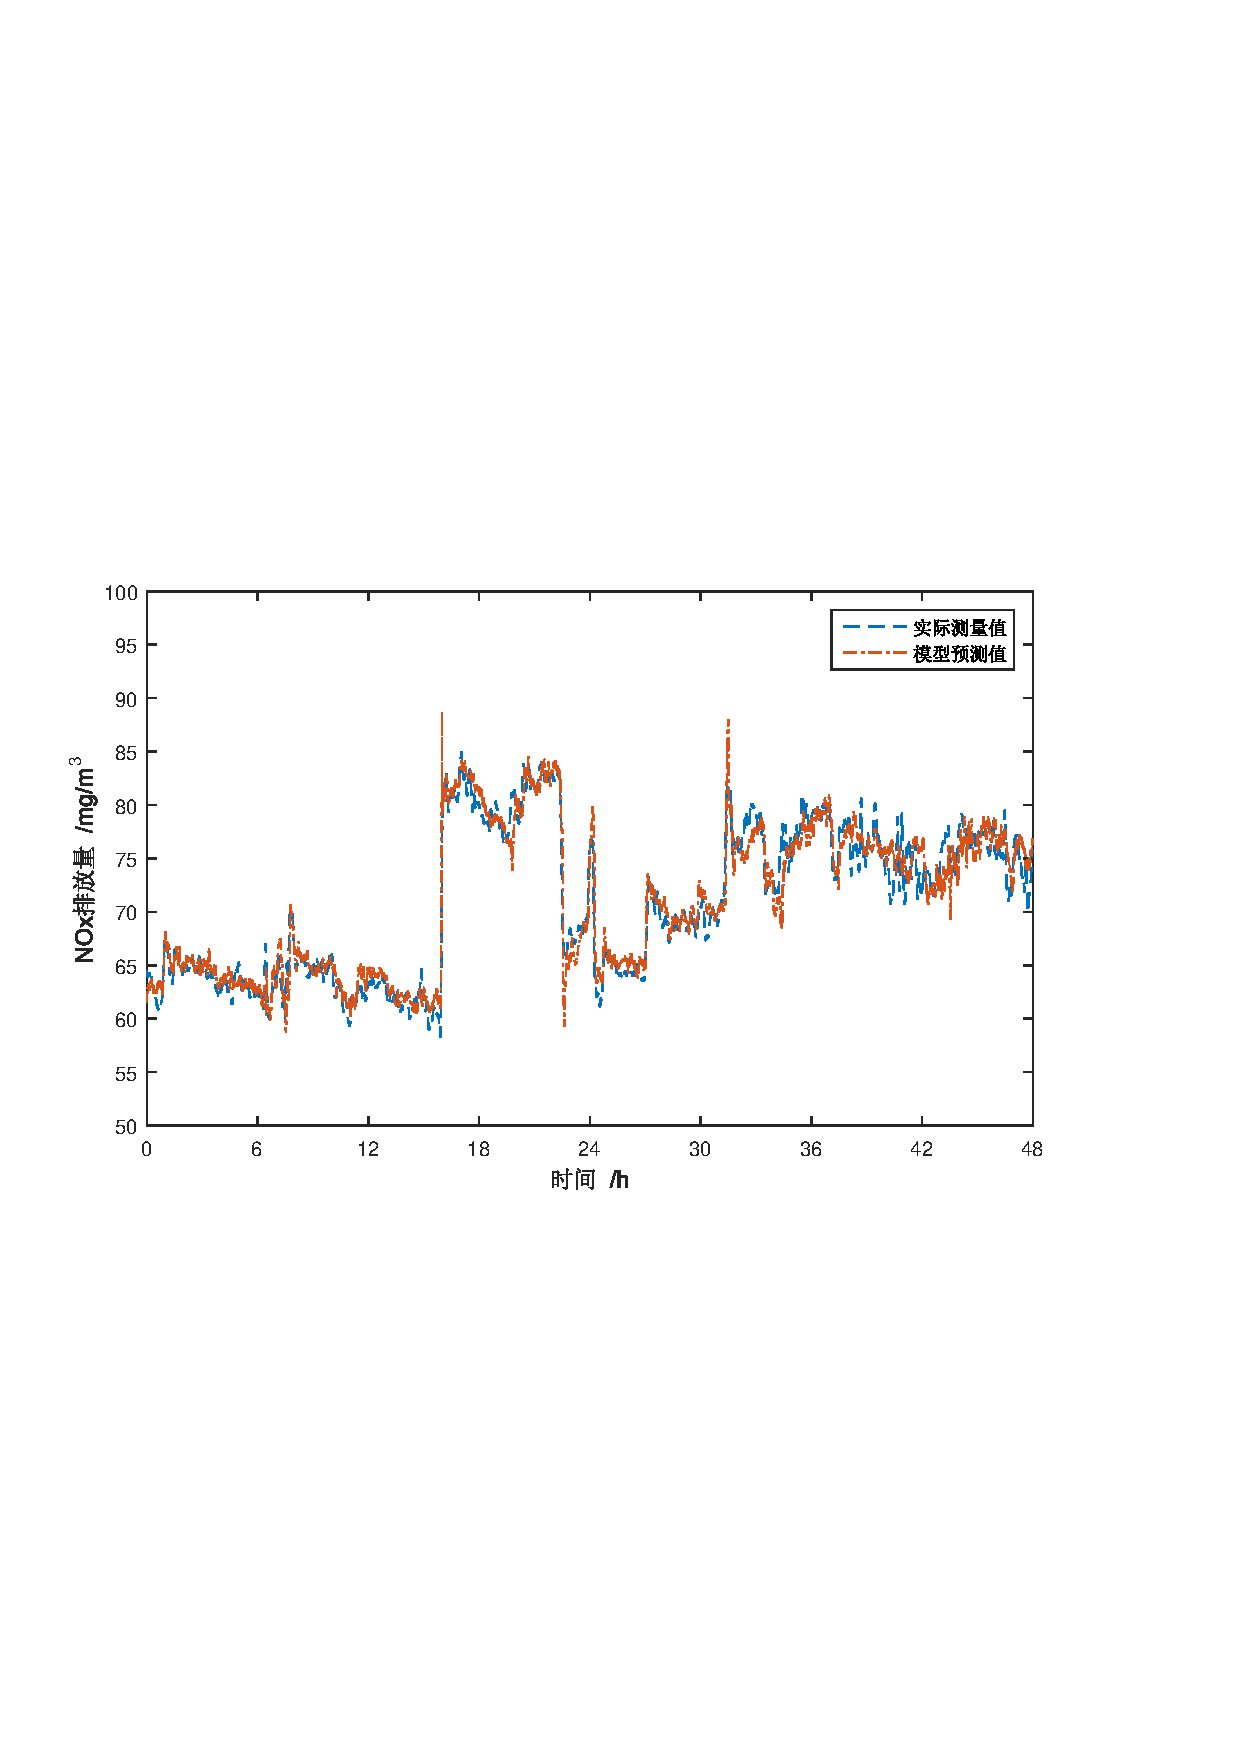
\includegraphics[width=13cm]{soft_sensor_res}
\caption{软测量模型预测效果} \label{fig:soft_sensor_res}
\end{figure}

\section{本章小结}
~\ce{NOx}~是锅炉排放的主要污染物之一,而目前采用的~\ce{NOx}~测量仪表经常出现故障,影响回路的自动控制投运率。为此,本章采用多元线性回归方法建立~\ce{NOx}~软测量模型,对~\ce{NOx}~排放量进行估计。为了让模型能够反映系统的工况变化,结合滚动窗设计了在线更新的软测量模型,并研究了滚动窗参数对模型的影响。另外,比较了不同自变量选择方法的效果,仿真结果显示基于BIC信息准则可以选出更符合实际要求的自变量。最后对比了软测量模型的估计值与现场实测值,结果表明结合滚动窗的软测量模型预测效果达到设计要求,且能在运行较长时间后保持精度不降低。

